\documentclass[10pt]{article}
\usepackage[ngerman]{babel}
\usepackage[utf8]{inputenc}
\usepackage[T1]{fontenc}
\usepackage{amsmath}
\usepackage{amsfonts}
\usepackage{amssymb}
\usepackage[version=4]{mhchem}
\usepackage{stmaryrd}
\usepackage{graphicx}
\usepackage[export]{adjustbox}
\graphicspath{ {./images/} }
\usepackage{bbold}

\title{Hauptprüfung Abiturprüfung 2022 - Leistungsfach }

\author{Alexander Schwarz\\
www.mathe-aufgaben.com}
\date{}


\begin{document}
\maketitle
 Baden-WürttembergJuni 2022

\section*{Aufgabe C1}
Ein Onlineshop bietet Patronen mit schwarzer Tinte und Patronen mit farbiger Tinte an.\\
a) Erfahrungsgemäß beträgt der Verkaufsanteil der Patronen mit schwarzer Tinte $65 \%$. Betrachtet wird eine zufällige Auswahl von 100 verkauften Patronen.\\
Es wird davon ausgegangen, dass dabei die Anzahl der Patronen mit schwarzer Tinte binomialverteilt ist. Bestimmen Sie die Wahrscheinlichkeit folgender Ereignisse:\\
A: „Genau 66 der verkauften Patronen sind mit schwarzer Tinte gefüllt."\\
B: „Die Anzahl der verkauften Patronen mit schwarzer Tinte weicht um mehr als 10\% vom Erwartungswert dieser Anzahl ab."\\
b) Im Folgenden werden nur Patronen betrachtet, die mit schwarzer Tinte gefüllt sind. Die Füllmenge einer solchen Patrone wird als normalverteilt mit dem Erwartungswert 8 ml und der Standardabweichung $0,04 \mathrm{ml}$ angenommen. Eine der beiden Abbildungen zeigt den Graphen der zugehörigen Dichtefunktion.\\
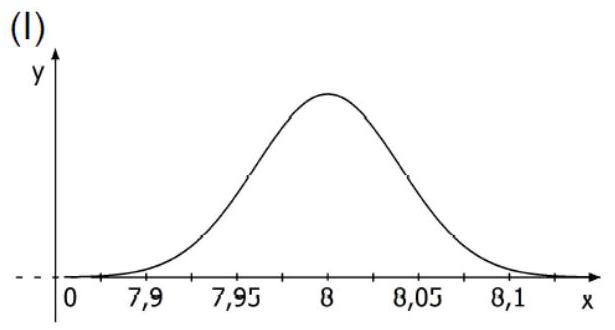
\includegraphics[max width=\textwidth, center]{2025_04_24_e3129e6cea71a3af61f3g-2(1)}\\
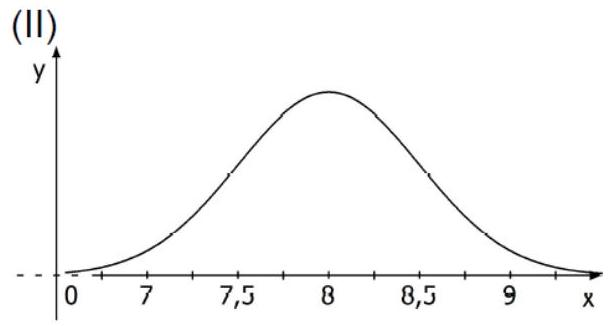
\includegraphics[max width=\textwidth, center]{2025_04_24_e3129e6cea71a3af61f3g-2}

Geben Sie die Abbildung an, die den Graphen der zugehörigen Dichtefunktion nicht zeigt, und begründen Sie Ihre Angabe.\\
Berechnen Sie die Wahrscheinlichkeit dafür, dass eine zufällig ausgewählte Patrone weniger als $7,95 \mathrm{ml}$ Tinte enthält.\\
Betrachtet wird das Ereignis, dass eine zufällig ausgewählte Patrone zwischen $7,98 \mathrm{ml}$ und $8,04 \mathrm{ml}$ Tinte enthält. Geben Sie ein anderes Ereignis im Sachzusammenhang an, welches exakt dieselbe Wahrscheinlichkeit hat. (1 VP)\\[0pt]
Bestimmen Sie das kleinste Intervall [a;b], so dass die Füllmenge einer zufällig ausgewählten Patrone mit einer Wahrscheinlichkeit von 92\% in [a;b] liegt.\\
c) Betrachtet wird die für $x \geq 0$ definierte Funktion $f$ mit $f(x)=0,25 \cdot e^{-0,25 x}$. Weisen Sie nach, dass $f$ eine Dichtefunktion über ihrem Definitionsbereich ist.

Die Zeitdauer in Stunden zwischen dem Eingang einer Bestellung im Onlineshop und dem Versand der Ware kann modellhaft durch eine stetige Zufallsgröße mit der Dichtefunktion $f$ beschrieben werden.\\
Mit einer Wahrscheinlichkeit von $85 \%$ wird eine Ware innerhalb von $t$ Stunden nach Eingang der Bestellung versandt. Bestimmen Sie den Wert von $t$.

\section*{Lösungen}
\section*{Aufgabe C1}
a) A: „Genau 66 der verkauften Patronen sind mit schwarzer Tinte gefüllt."

B: „Die Anzahl der verkauften Patronen mit schwarzer Tinte weicht um mehr als 10\% vom Erwartungswert dieser Anzahl ab."

X = Anzahl der verkauften Patronen mit schwarzer Tinte.\\
X ist binomialverteilt mit $\mathrm{n}=100$ und $\mathrm{p}=0,65$.\\
$\mathrm{P}(\mathrm{A})=\mathrm{P}(\mathrm{X}=66) \approx 0,082$\\
Erwartungswert der Anzahl: $\mathrm{E}(\mathrm{X})=\mathrm{n} \cdot \mathrm{p}=100 \cdot 0,65=65$\\
10\% vom Erwartungswert sind 6,5.

$$
\begin{aligned}
& P(B)=P(X<65-6,5)+P(X>65+6,5)=P(X \leq 58)+P(X \geq 72) \\
& P(X \leq 58)+1-P(X \leq 71) \approx 0,0877+1-0,9152=0,1725
\end{aligned}
$$

b) Geben Sie die Abbildung an, die den Graphen der zugehörigen Dichtefunktion nicht zeigt, und begründen Sie Ihre Angabe.

Wegen $\mu=8$ und $\sigma=0,04$ sind die Wendestelle der Dichtefunktion bei $\mathrm{x}_{1}=\mu-\sigma=8-0,04=7,96$ und $\mathrm{x}_{2}=\mu+\sigma=8+0,04=8,04$.\\
Daher zeigt die Abbildung (II) nicht die Dichtefunktion.\\
Berechnen Sie die Wahrscheinlichkeit dafür, dass eine zufällig ausgewählte Patrone weniger als $7,95 \mathrm{ml}$ Tinte enthält.\\
$\mathrm{Y}=$ Füllmenge der ausgewählten Patrone in ml\\
Y ist normalverteilt mit $\mu=8$ und $\sigma=0,04$\\
$\mathrm{P}(\mathrm{Y}<7,95) \approx 0,106$

Betrachtet wird das Ereignis, dass eine zufällig ausgewählte Patrone zwischen $7,98 \mathrm{ml}$ und $8,04 \mathrm{ml}$ Tinte enthält. Geben Sie ein anderes Ereignis im Sachzusammenhang an, welches exakt dieselbe Wahrscheinlichkeit hat.\\
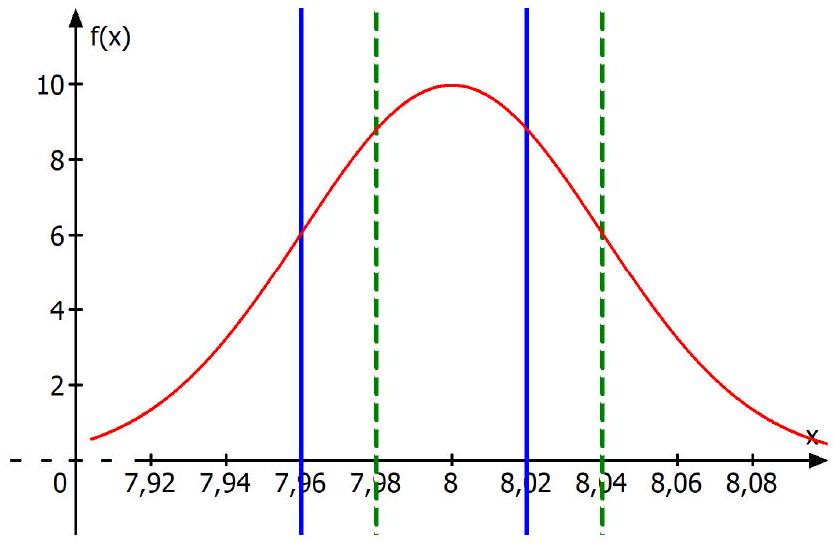
\includegraphics[max width=\textwidth, center]{2025_04_24_e3129e6cea71a3af61f3g-3}

Da das Schaubild der Dichtefunktion symmetrisch zur senkrechten Geraden x=8 ist, ist der Flächeninhalt im Intervall $[7,98 ; 8,04]$ gleich groß wie der Flächeninhalt im Intervall [7,96;8,02].

Ereignis: Eine zufällig ausgewählte Patrone enthält zwischen 7,96 ml und 8,02 ml Tinte.

Bestimmen Sie das kleinste Intervall [a;b], so dass die Füllmenge einer zufällig ausgewählten Patrone mit einer Wahrscheinlichkeit von 92\% in [a;b] liegt.

Da das Intervall [a;b] möglichst klein sein soll, muss es symmetrisch um den Erwartungswert $\mu$ liegen, da die Fläche um den Erwartungswert zwischen der Dichtefunktion und der x-Achse am größten ist.

Bedingung: $P(8-z \leq X \leq 8+z)=0,92$\\
Für $z=0,07$ gilt $\mathrm{P}(7,93 \leq X \leq 8,07) \approx 0,92$.\\
Somit ist $\mathrm{a} \approx 7,93$ und $\mathrm{b} \approx 8,07$.\\
c) Weisen Sie nach, dass feine Dichtefunktion über ihrem Definitionsbereich ist.\\
1.Bedingung: $f(x) \geq 0$ für $x \geq 0$

Es gilt $f(x)=0,25 \cdot e^{-0,25 x}>0$, da $e^{-0,25 x}>0$ ist für alle $x \in \mathbb{R}$\\
2.Bedingung: $\int_{0}^{+\infty} f(x) d x=1$\\
$\int_{0}^{u} f(x) d x=\left[0,25 \cdot \frac{1}{-0,25} e^{-0,25 x}\right]_{0}^{u}=-e^{-0,25 u}+e^{0}=1-e^{-0,25 u}$\\
Für $u \rightarrow+\infty$ gilt $1-\mathrm{e}^{-0,25 u} \rightarrow 1$\\
Da die Funktion $f$ beide Bedingungen erfüllt, ist sie eine Dichtefunktion.

Mit einer Wahrscheinlichkeit von $85 \%$ wird eine Ware innerhalb von $t$ Stunden nach Eingang der Bestellung versandt. Bestimmen Sie den Wert von t.

Bedingung: $\int_{0}^{t}\left(0,25 \cdot e^{-0,25 x}\right) d x=0,85$\\
$\int_{0}^{t}\left(0,25 \cdot e^{-0,25 x}\right) d x=\left[-e^{-0,25 x}\right]_{0}^{t}=-e^{-0,25 t}+1$\\
$-e^{-0,25 t}+1=0,85$\\
$\Leftrightarrow t=\frac{1}{-0,25} \ln (0,15) \approx 7,59$


\end{document}